\documentclass[a4paper,twocolumn,oneside,bibtotoc,smallheadings,pointlessnumbers,halfparskip,DIV15]{scrartcl}
% tocleft,
\usepackage[pdftex]{graphicx}
\usepackage[ngerman]{babel}
\usepackage[utf8]{inputenc}
\usepackage{../../assets/uniinput}
\usepackage[T1]{fontenc}
\usepackage{amssymb,amsmath}
\usepackage{booktabs}
\usepackage{enumerate}
\usepackage{siunitx}
\sisetup{
	seperr		=	true,
	trapambigerr	=	true,
	openerr		=	(,
	closeerr	=	),
	expproduct	=	cdot,
	padnumber	=	both,
	stickyper	=	true,
	per		=	slash,
	trapambigfrac	=	true,
	repeatunits	=	false,
	openfrac	=	(,
	closefrac	=	),
	prefixsymbolic 	=	true,
	prefixproduct	=	cdot,
	decimalsymbol	=	comma,
        tabnumalign     =       left,
        tabtextalign    =       left
}
\usepackage{color}
\definecolor{grey}{rgb}{.4,.4,.4}
\definecolor{darkgreen}{rgb}{0,.35,0}
\definecolor{ltgray}{gray}{0.90}
% \definecolor{darkblue}{rgb}{0,0,.6}
% \definecolor{darkred}{rgb}{.6,0,0}
% \definecolor{red}{rgb}{.98,0,0}
\usepackage{listings}
\lstdefinelanguage{Maxima}{
  keywords={addrow,addcol,zeromatrix,ident,augcoefmatrix,ratsubst,diff,ev,tex,%
    with_stdout,nouns,express,depends,load,submatrix,div,grad,curl,%
    rootscontract,solve,part,assume,sqrt,integrate,abs,inf,exp,float},
  sensitive=true,
  comment=[n][\itshape]{/*}{*/}
}
\lstset{language=C++,
%   commentstyle=\itshape\color{darkgreen},
%   commentstyle=\color{darkgreen},
%   keywordstyle=\bfseries, %\color{darkblue},
%   stringstyle=\color{darkred},
%   basicstyle=\ttfamily\scriptsize,
  morekeywords={TH1F,TLorentzVector,TVector3,vector,TFile,TFitResultPtr,TF1,\
                TGraph,TH1,TObject,TCanvas,string,Double_t,TGraphErrors},
  basicstyle=\scriptsize,
  numbers=left,
  numberstyle=\tiny,%\color{gray},
  stepnumber=1,
  tabsize=4,
  showspaces=false,
  showstringspaces=false,
  breaklines=true,
  frame=lrtb,
  captionpos=b,
  extendedchars=true,
  inputencoding=utf8,
%   backgroundcolor=\color{ltgray}
}
\usepackage[pdftex]{hyperref}
\hypersetup{
% 	colorlinks	=	true,
% 	urlcolor	=	darkblue,
	pdftitle	=	{Protokoll zum F-Praktikumsversuch 'Compton-Effekt'},
	pdfsubject	=	{Praktikumsversuch}
	pdfauthor	=   	{robert.riemann@physik.hu-berlin.de,thomas.murach@physik.hu-berlin.de},
	pdfkeywords	=	{Fortgeschrittenen-Praktikum,Praktikumsversuch, 2010, Compton-Effekt}
% 	pdfcreator	=	{pdftex},
% 	pdfproducer	=	{pdftex}
}

\newcommand{\dd}[1]{\mathrm{d}#1\,} % declare dx operator, usage: \dd{x} for dx
\newcommand{\lref}[1]{Listing (\ref{lst:#1})} % refer to a listing, usage: \lref{label} for Listing (...)
\newcommand{\fref}[1]{Abb. (\ref{fig:#1})} % refer to a figure, usage: \lref{label} for Abb. (...)
\newcommand{\tref}[1]{Tab. (\ref{tab:#1})} % refer to a table, usage: \lref{label} for Tab. (...)
\newcommand{\eref}[1]{Gl. (\ref{eqn:#1})} % refer to a equation, usage: \lref{label} for Tab. (...)


\begin{document}
% % % % % % % % % % % % % % % % % % % % % % % % 
\title{{\centering \rule{15cm}{0.001cm}\\
\Large{\textsc{Institut für Physik der
Humboldt-Universität zu Berlin}}}\\ \centering \rule{15cm}{0.001cm}\\
\vspace{15mm} \centering

\includegraphics[scale=0.9]{../../assets/siegel}\\
\vspace{18mm}
{\bf{\huge{Fortgeschrittenen-Praktikum}}}\\
Versuchsprotokoll\\
\vspace{14mm}
Compton-Effekt\\
\vspace{14mm} {\small{\textbf{Betreuer: M. zur Nedden}}}\\}
\author{Robert Riemann; Matr.Nr.: 521085\\
Thomas Murach; Matr.Nr.: 517771\vspace{18mm}}
\vspace{18mm}
% \date{15. Juni 2008}
% % % % % % % % % % % % % % % % % % % % % % % %
\onecolumn
\maketitle
\twocolumn

\tableofcontents
\listoffigures
\listoftables

\section{Voraussetzungen}

\subsection{Versuchsziel}

In diesem Versuch sollte die Lebensdauer von Myonen vermessen werden. Dafür
wurden verschiedene Logikschaltungen aufgebaut, mit denen die mit
Szintillationszählern registrierten Signale untersucht werden konnten. Aus dem
resultierenden Zeit-Intensitäts-Spektrum kann man dann die Halbwertszeit
ableiten.

\subsection{Physikalische Grundlagen}

Die hier untersuchten Teilchen stammen aus der kosmischen Höhenstrahlung. Aus dem Weltall zur Erde gelangende Protonen wechselwirken mit Atomkernen der
oberen Atmosphäre, woraufhin ein Teilchenschauer entsteht, der hauptsächlich
aus Pionen besteht. Die geladenen $π^{\pm}$ wiederum zerfallen nach
\cite[Gl.16]{script} größtenteils in
$μ^{\pm}$ und die dazugehörigen (Anti-) Neutrinos:
\begin{eqnarray}
π^+ &\rightarrow& μ^+ + ν_μ\\
π^- &\rightarrow& μ^- + \overline{ν}_μ
\end{eqnarray}
Diese Myonen besitzen eine Lebensdauer von ca. \SI{2}{\micro\second} und
üblicherweise eine Geschwindigkeit, die fast der Lichtgeschwindigkeit
entspricht. Nach klassischer Rechnung würden die Myonen im Schnitt also nur
etwa 600m weit kommen, aber durch die relativistische Zeitdilatation, die die
Myonen von der Erde aus gesehen erfahren, gelangen sie trotzdem bis zu uns.

Die Myonen selbst zerfallen wiederum fast ausschließlich wie folgt (s.
\cite[Gl.5]{script}):
\begin{eqnarray}
μ^+ &\rightarrow& e^+ + ν_l + \overline{ν}_μ\\
μ^- &\rightarrow& e^- + \overline{ν}_e + ν_μ
\end{eqnarray}
Dabei liegt die Halbwertszeit $τ_μ$ nach \cite[Gl.4]{script} bei
\begin{equation}
τ_μ = \SI{2,19703(4)}{\micro\second} 
\label{eqn:tau_mu_theo}
\end{equation}
Diese Größe werden wir versuchen zu verifizieren.

\subsection{Versuchsaufbau}

Der Detektoraufbau, der in \fref{detector} dargestellt ist, wurde
\cite[Abb.3]{script} entnommen.
\begin{figure}[htb]
     \centering
     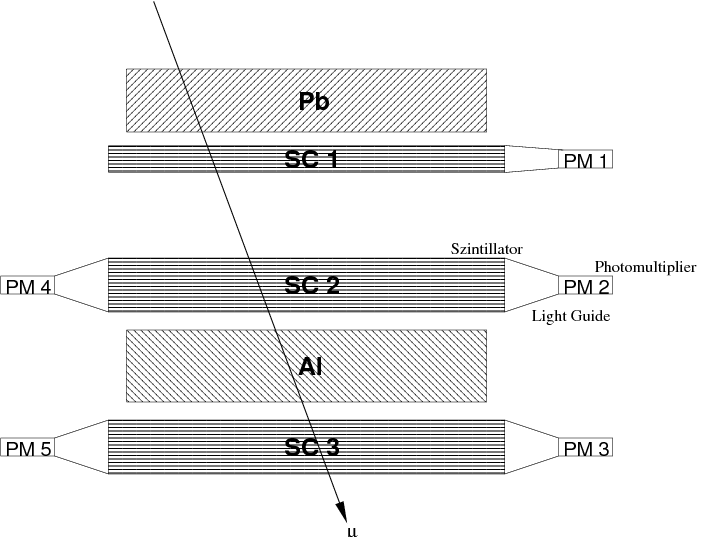
\includegraphics[width=1\columnwidth,keepaspectratio]{../docs/detector.png}
     \caption{Detektoraufbau}
     \label{fig:detector}
\end{figure}
Man kann in diesem Bild erkennen, dass sich oben über dem ersten
Szintillationszähler SC1 ein großer Bleiblock befindet, der dafür sorgt, dass
von oben keine anderen Teilchen außer Myonen den Detektor erreichen. Dies
funktioniert, da alle anderen Teilchen beim Durchgang durch Materie entweder
mehr Energie durch Bremsstrahlung oder durch Ionisationsverluste verlieren als
Myonen es tun. Der Szintillationszähler SC1 registriert also die eintreffenden
Myonen, und da diese annähernd Lichtgeschwindigkeit besitzen, werden sie auch
im Rahmen der Detektor-Zeitauflösung zeitgleich im Szintillationszähler SC2
registriert. Anschließend müssen die Teilchen einen Aluminiumblock passieren,
der sie so stark abbremst, dass man davon ausgehen kann, dass sie zur Ruhe
gekommen sind. In SC3 sollte also zunächst kein Signal beobachtet werden. Die
Myonen, die wir selektieren möchten, zerfallen also zwischen SC2 und SC3. Das
beim Zerfall ausgesendete (Anti-) Elektron muss mit einer Zeitverzögerung in
SC3 detektiert werden (es wäre auch möglich, dass es in SC2 gemessen wird, aber
unsere Logikschaltung selektiert nur den ersten Fall.)

Um die erwähnten (Anti-) Koinzidenzen zu gewährleisten, haben wir Abfolgen von
UND- und ODER-Schaltungen verwendet.

Wie in vielen Experimenten muss man versuchen, den Untergrund zu minimieren.
Eine von uns umgesetzte Methode ist die Forderung einer Koinzidenz in den
beiden zu einem Szintillationszähler gehörenden Photomultipliern (PM 2 und PM 4
für SC2 und PM 3 und PM 5 für SC3). Dies reduziert den Einfluss von zufällig in
den Photomultipliern thermisch ausgelösten Elektronen, da diese kaum
gleichzeitig in beiden PMs auftreten werden.

\subsection{Verwendete Geräte}

Für die Versuchsdurchführung wurde der im \cite{script} vorgeschlagenen und
bereits vorbereitete Aufbau verwendet. Das wären im Einzelnen die folgenden
Geräte:
\begin{itemize}
\item Plastikszintillatoren NE102A
\item Photomultiplier H7360-02
\item Koaxialkabel RG58U
\item Liste der NIM- und Elektronikmodule: s. \cite[Anhang B]{script}
\end{itemize}
\section{Bestimmung des hadronischen Wirkungsquerschnitts $\sigma_0^{Had}$}
\subsection{Selektion der hadronischen Ereignisse}
Wir haben mehrere Datensamples zu Verfügung gehabt. Zunächst waren dort die gemessenen L3-Daten, die bei verschiedenen Schwerpunktenergien aufgenommen wurden (bei 89.48 GeV, 91.33 GeV und 93.02 GeV). Die integrierten Luminositäten unterscheiden sich auch und wurden in \cite[S.9]{script} gegeben; außerdem konnten wir mit zwei Monte-Carlo-Daten arbeiten, die uns der aktuellen Theorie entsprechende Verteilungen von Hadronen und Myonen gab. Mit diesen Simulationsdaten konnten wir also überprüfen, welche Wirkung unsere Cuts auf den jeweiligen $Z^0$-Zerfallskanal hatten. So konnten wir feststellen, dass bei hadronischen Ereignissen immer mindestens ca. 9 Cluster (separierte Einträge im Kalorimeter) Teilchen detektiert haben. Daraus ließ sich ein wirksamer Cut gewinnen, der unter anderem die meisten Myonen-Ereignisse nicht zulässt. Ein weiterer Cut wurde angewendet, indem verlangt wurde, dass die (sichtbare) Energie eines Events mehr als $70\%$ der Schwerpunktsenergie beträgt. Zum Beispiel zerfallen $\tau$-Leptonen oft so, dass die Art und Anzahl der Teilchen, die in die Kalorimeter gelangt, sehr einem hadronischen Ereignis ähnelt. Allerdings wird dabei viel Energie an dabei entstehende Neutrines abgegeben, die nicht registriert werden können, sodass die sichtbare Energie in einem solchen Fall wesentlich kleiner ist. Mit diesem Cut können demnach viele $\tau$-Zerfälle ausgeschlossen werden. Dabei haben wir auch immer darauf geachtet, dass die Effizienz unserer Cuts nicht zu klein wird. Mit den eben erwähnten Cuts gelang es uns, eine Effizienz von
\begin{eqnarray}
\epsilon_{had} &=& \frac{9770 \pm \sqrt{9770} \pm 158}{10000}\\
&=& 0.98 \pm 0.01 \pm 0.02
\end{eqnarray}
zu erreichen. Dabei ist der erste angegebene Fehler der statistische Fehler und der zweite ist der systematische Fehler, der aus der ''willkürlichen'' Wahl der Schnittkriterien resultiert. Wenn man diese Cuts allerdings auf das Myonen-Monte-Carlo-Sample anwendet, so werden nur 19 hadronische Events erkannt (bei 9970 Events im Sample!). Die Fehlerquote durch Myonenereignisse ist also sehr gering. Unsere Schnitte sind also offenbar gut geeignet, um Hadronen-Events aus den Daten zu selektieren.

\subsection{Berechnung der hadronischen Wirkungsquerschnitte bei verschiedenen $\sqrt{s}$}
Die eben besprochenen Schnitte haben wir nun auf die Messdaten angewandt. Dabei kamen die in \tref{hadronic_xsecs} gezeigten Werte heraus. Die angegebenen Fehler sind wiederum statistischer und dann systematischer Fehler. Diese Konvention verwenden wir im gesamten folgenden Protokoll.\\
Der Fehler des Wirkungsquerschnitts ergibt sich durch Fehlerfortpflanzung aus den jeweiligen Fehlern von N und von $\epsilon_{had}$.

\begin{table}[htbp]
\centering
\setlength{\tabcolsep}{14pt}
\begin{tabular*}{\columnwidth}{%
S[tabformat=2.1]%
S[tabformat=2.2]%
S[tabformat=1.2]}
\toprule
{Energie / GeV} &
{Zahl N der analysierten Hadronen-Ereignisse} &
{Wirkungsquerschnitt $\sigma_0^{Had}$ / nb}\\
\midrule
89.48 & {$1848 \pm 43 \pm 52$} & {$10.55 \pm 0.18 \pm 0.16$} \\
91.33 & {$3980 \pm 63 \pm 79$} & {$29.98 \pm 0.49 \pm 0.43$} \\
93.02 & {$2149 \pm 46 \pm 51$} & {$14.56 \pm 0.24 \pm 0.24$} \\
\bottomrule
\end{tabular*}
\caption{experimentelle Messung der Ein- und Ausgangswiderstände}
\label{tab:hadronic_xsecs}
\end{table}

Diese Wirkungsquerschnitte kann man nun in das bereitgestellte Fit-Programm einsetzen. Dieses Programm wurde von uns leicht verändert und kann im Anhang unter ??BLABLA?? gefunden werden. Unter Berücksichtigung der statistischen Fehler von N, $\epsilon_{had}$ und der Luminosität (deren Fehler war in \cite[S.9]{script} mit $1\%$ des gegebenen Wertes angegeben) kann der statistische Fehler von $\sigma_0$ und mit den systematischen Fehlern von N und $\epsilon_{had}$ durch dieses Programm berechnet werden. Für den gesamten hadronischen Wirkungsquerschnitt resultiert also:
\begin{eqnarray}
\sigma_0^{Had} = 40.33 \pm 0.65 \pm 0.27
\end{eqnarray}
% \section{Diskussion der Ergebnisse}
Die fundamtentalen Ergebnisse dieses Versuchs werden in diesem Abschnitt noch einmal mit den theoretisch bzw. experimentell ermittelten Literaturwerten zu verglichen. Diese Zahlen wurden dem \cite{pdb} entnommen.\\
Zunächst haben wir die Masse des Z-Bosons bestimmt. Dieses Ergebnis weicht um gerade einmal \si{0.03}{\percent} vom gegebenen Wert ab, der \si{91.1876}{\giga\electronvolt} beträgt. Dabei muss man erwähnen, dass für die Fit-Parameter ohne die von uns nicht nachvollziehbare QCD-Korrektur sicherlich nicht so gut mit den realen Werten übereinstimmen würden.\\
Die totale Zerfallsbreite weicht vom realen Wert (\si{2.4952}{\giga\electronvolt}) um immerhin \si{4}{\percent} ab. Somit ist auch die Abweichung der Lebensdauer genauso groß. Ein Vergleich der Partialbreiten ist in \tref{partial} zu finden.
\begin{table*}[ht]
\begin{tabular*}{0.6\textwidth}{%
S[tabformat=2.1]%
l%
l}
\toprule
{$\Gamma_{l,\mathrm{theo}}$ [\si{GeV}]} &
{$\Gamma_{l,\mathrm{exp}}$ [\si{GeV}]} &
{relative Abw. [\si{\percent}]}\\
0.083 & 0.084 & 1\\
\midrule
{$\Gamma_{{\nu_l},\mathrm{theo}}$ [\si{GeV}]} &
{$\Gamma_{{\nu_l},\mathrm{exp}}$ [\si{GeV}]} &
{relative Abw. [\si{\percent}]}\\
0.166 & 0.499 & 200\\
\midrule
{$\Gamma_{\mathrm{Had,theo}}$ [\si{GeV}]} &
{$\Gamma_{\mathrm{Had,exp}}$ [\si{GeV}]} &
{relative Abw. [\si{\percent}]}\\
1.86 & 1.74 & 6\\
\bottomrule
\end{tabular*}
\caption{Zahl der analysierten Hadronen-Ereignisse und zugehörige Wirkungsquerschnitte bei verschiedenen Schwerpunktsenergien}
\label{tab:partial}
\end{table*}
Offenbar weichen die Partialbreiten nur um einige Prozent ab, allerdings gibt es große Abweichungen bei der Neutrino-Partialbreite. Allerdings ist in der Gleichung für diese Größe abgesehen von Konstanten nur die Masse einzusetzen, und die ist in unserem Experiment beinahe korrekt. Also ist diese Abweichung kein Produkt unserer Daten-Unsicherheiten, sondern eher eine Schwäche der Theorie, die zu der verwendeten Formel führt. Man sollte dabei noch erwähnen, dass  in \cite{pdb} nur eine Partialbreite für ``unsichtbare'' Events angegeben ist, wobei nicht einsichtig ist, ob dabei noch andere Ereignisse als Neutrinoevents erfasst wurden. Dies wäre natürlich die naheliegendste Erklärung für die Unstimmigkeiten.\\
Der schwache Mischungswinkel (in \cite{pdb} als $\sin^2\Theta_W$ bezeichnet) weicht um gerade einmal 0.4\si{\percent} vom gegebenen Wert ($\sin^2\Theta_W = 0.231$) ab.\\
Schließlich ist noch der Farbfaktor zu betrachten. Der Theoriewert liegt bei 3.0, während wir einen Wert von $3.2\pm 0.13$ erreichten (relative Abweichung: 6\si{\percent}). Auf jeden Fall ist 3 die sicherlich naheliegendste Antwort auf die Frage, welche Zahl von Quarkfamilien es gibt.\\
Alle Abweichungen von den realen Werten resultieren aus der Ungenauigkeit der Selektion sowie aus der Unsicherheit des Detektors selbst, was man schon an der Tatsache sehen konnte, dass es gemessene Energien von deutlich mehr als der Schwerpunktsenergie gab. Es böte sich zum Beispiel an, weitere Cut-Kriterien einzuführen, wie zum Beispiel Shape-Variablen. Damit kann man sehr gut zwischen Hadronen und nicht-Hadronen unterscheiden, allerdings übersteigt dies die Moglichkeiten innerhalb dieses Praltikumsversuchs. Wenn man also besser selektieren könnte, wäre die systematische Abweichung der Ergebnisse verbessert. Allerdings sind die statistischen Fehler oft etwas größer, sodass man hier ebenfalls Verbesserungen vornehmen müsste. Die naheliegendste Variante wäre das Verwenden einer besseren Statistik, also die Betrachtung von mehr Events. Außerdem waren die Monte Carlo-Daten nicht in verschiedene Samples für die vorliegenden Schwerpunktsenergien aufgeteilt, was natürlich ebenfalls die dominierenden Prozesse und deren quantitatives Verhältnis beeinflusst. Was sicherlich in einer tiefergehenden Studie zu betrachten wäre, ist die (bisher vernachlässigte) Zahl der Untergrundereignisse. Dies ist mit Sicherheit nicht korrekt, aber da uns keine Möglichkeit zur Verfügung stand, Informationen zu gewinnen, die über eine mutmaßende Spekulation hinausgehen, haben wir uns entschieden, den Untergrund zu vernachlässigen.
\renewcommand{\refname}{Literatur und Programme}
\begin{thebibliography}{xxxxxx}
\bibitem[Skript]{script}
Dobbert, Julia, Anleitung zum Versuch ``Leitfähigkeit und Hall-Effekt'' im Fortgeschrittenen-Praktikum, Humboldt–Universität, 2008
\bibitem[PDB]{pdb}
Particle Data Group, Particle Physics Booklet, Physics Letters, 2008
\bibitem[Barlow]{barlow}
Barlow, R. J., Statistics, Manchester University, Wiley Verlag, 1999
\bibitem[ROOT]{root}
ROOT Version 5.26/00, 2009, \href{http://root.cern.ch}{http://root.cern.ch}
\bibitem[maxima]{maxima}
Maxima Version 5.19.2, 2009, \href{http://maxima.sourceforge.net}{http://maxima.sourceforge.net}
\end{thebibliography}
\appendix
\section{Abschwächung des Lasers}
\label{sec:laser}
In der folgenden Rechnung wird berechnet, wie stark das Laserlicht abgeschwächt
werden muss, damit mit \SI{99,9}{\percent}iger Wahrscheinlichkeit nur ein
einziges Photon pro Puls an der Photodiode ankommt. Dafür wird verwendet, dass
die Photonenzahl beim Laser einer Poisson-Statistik unterliegt. Zunächst muss
berechnet werden, wie viele Photonen sich in einem Puls befinden (Photonenzahl
$N_P$), und anschließend kann bestimmt werden, um welchen Faktor die Intensität
verringert werden muss, um die genannte Wahrscheinlichkeit zu erreichen, nur ein
einziges Photon zu detektieren.
\begin{eqnarray}
E_{\mathrm{Puls}} &=& \SI{50}{mW}\cdot\SI{10}{ns} = \SI{50e-12}{J}\\
E_{\mathrm{Photon}} &=& hν = h\frac{c}{λ}\\
N_P &=& \frac{E_{\mathrm{Puls}}}{E_{\mathrm{Puls}}} = \SI{1,6e8}{}
\end{eqnarray}
Dies entspricht dem Erwartungswert λ der Photonenanzahl.
\begin{eqnarray}
P_λ(X=k) &=& \frac{λ^k}{k!}\mathrm{e}^{-λ}\\
\rightarrow P_{cλ}(1) &=& cλ\cdot\mathrm{e}^{-cλ} = \SI{0.999}{}
\end{eqnarray}
Hierbei ist $c$ eine Konstante, die beschreibt, welcher Anteil des Lichts die
Filter passieren soll. Diese Gleichung kann numerisch gelöst werden, wobei sich
hier das folgende für $c$ ergibt:
\begin{equation}
c = \SI{1.2e6}{}
\end{equation}
Wenn also die Filter so gewählt werden, dass die Intensität um einen Faktor von
ca. $10^6$ verringert wird, kann man davon ausgehen, dass nur ein Photon eines
Pulses den Detektor erreicht.

\section{Wahl der Polarisation}
\label{sec:zirkular}
Hier wird gezeigt, dass es möglich ist, als mögliche Polarisationszustände eine
horizontale, vertikale, rechts- und linkszirkulare Polarisation zu verwenden.
Dafür muss gezeigt werden, dass die zur gleichen Basis gehörenden Zustände
orthogonal zueinander sind, während die Zustände, die zu unterschiedlichen
Basen gehören, nicht orthogonal zueinander sein sollen.
\begin{eqnarray}
| \circlearrowright \rangle &=& \frac{1}{\sqrt{2}}(|\rightarrow\rangle +
i|\uparrow\rangle)\\
| \circlearrowleft \rangle &=& \frac{1}{\sqrt{2}}(|\rightarrow\rangle -
i|\uparrow\rangle)\\
\langle\uparrow|\uparrow\rangle &=& 1\\
\langle\uparrow|\rightarrow\rangle &=& 0\\
\langle\circlearrowleft|\circlearrowleft \rangle &=& 1\\
\langle\circlearrowleft|\circlearrowright \rangle &=& 0\\
|\langle\uparrow|\circlearrowleft \rangle| &=&
\left|\frac{1}{\sqrt{2}}\langle\uparrow|(|\rightarrow\rangle -
i|\uparrow\rangle\right|\\
 &=& \frac{1}{\sqrt{2}}\\
|\langle\uparrow|\circlearrowright \rangle| &=& \frac{1}{\sqrt{2}}\\
|\langle\rightarrow|\circlearrowleft \rangle| &=&
\left|\frac{1}{\sqrt{2}}\langle\rightarrow|(|\rightarrow\rangle -
i|\uparrow\rangle\right|\\
 &=& \frac{1}{\sqrt{2}}\\
|\langle\rightarrow|\circlearrowright \rangle| &=& \frac{1}{\sqrt{2}}
\end{eqnarray}
Man kann erkennen, dass die Skalarprodukte der beiden zur jeweils gleichen
Basis gehörenden Polarisationen für orthogonal zueinander stehende
Polarisationen null werden, was zu einer deterministischen Messung bei der Wahl
gleicher Basen von Alice und Bob führt. Andererseits sind die Skalarprodukte
von zu unterschiedlichen Basen gehörenden Polarisationen vom Betrage her immer
$1/\sqrt{2}$, sodass gar keine Aussage über den Polarisationszustand getroffen
werden kann, wenn die beiden unterschiedliche Basen verwenden. Somit ist
gezeigt, dass die in unserem Experiment getroffene Wahl einer orthogonalen,
linear-polarisierten und einer zirkular-polarisierten Basis für den Zweck der
quantenkryptographischen Schlüsselübertragung geeignet ist.

\onecolumn
\section{Messprotokoll}
\label{sec:protokoll}
\begin{figure}[!ht]
        \centering
        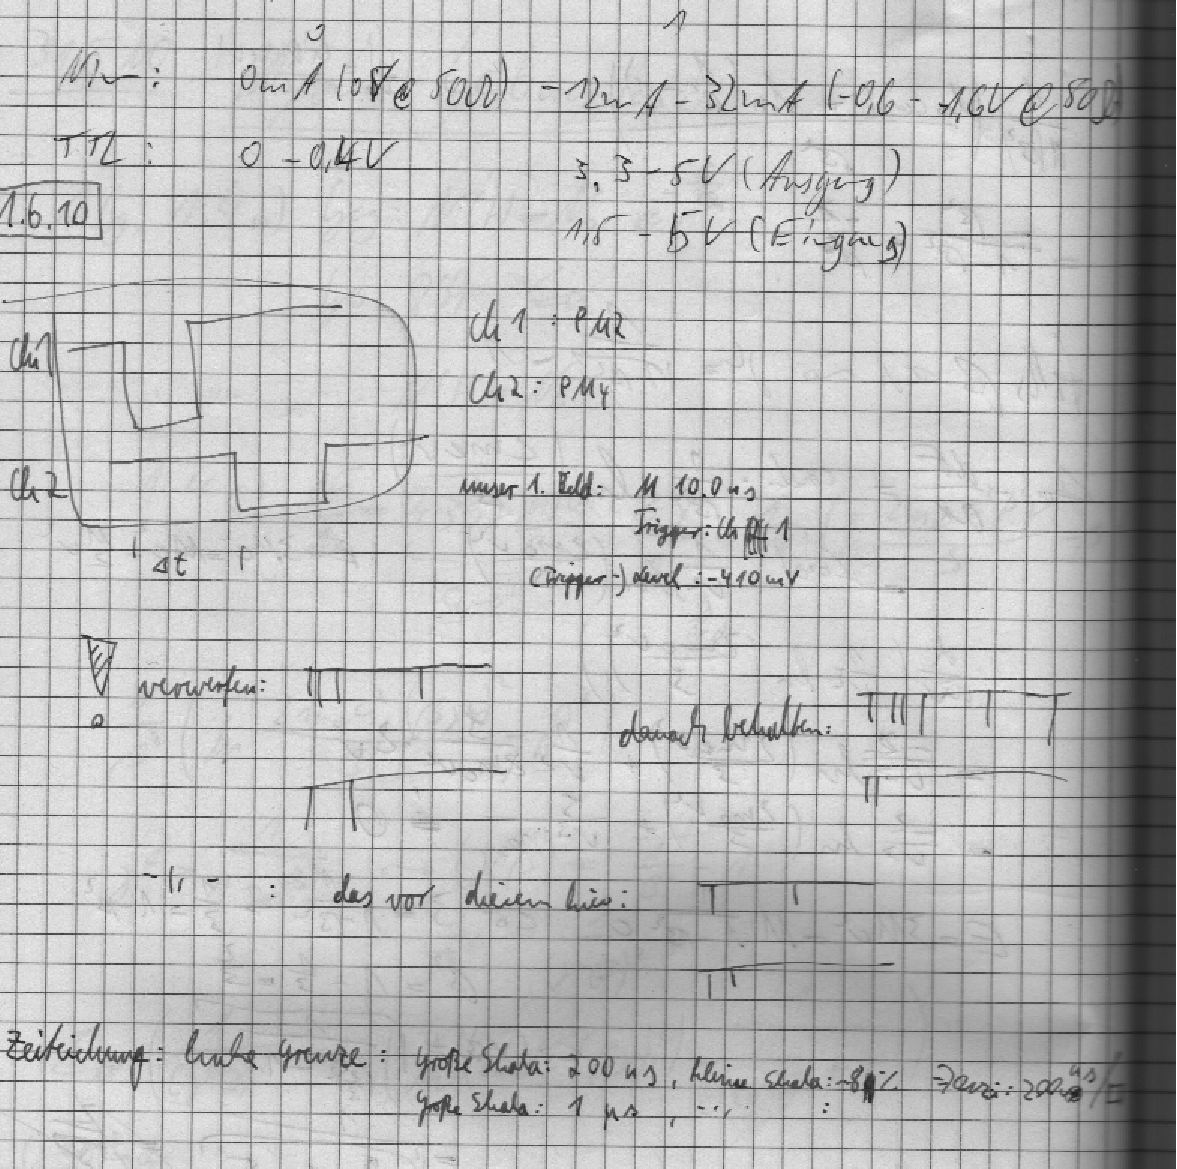
\includegraphics[page=1,width=.88\textwidth,keepaspectratio]{../data/messprotokoll}
%         \caption{Messprotokoll}
        \label{fig:protokoll}
\end{figure}

% \section{Beispiele}
% blabla
% 
% Weitere Information sind der Versuchsbeschreibung im \cite{script} zu entnehmen.
% 
% \begin{eqnarray}
% 	g &=& \SI{9.8157(11)}{\metre\per\second\squared} \\
%         \left[ g \right] &=& \si{\metre\per\Square\second} % großschreibung!
% 	\label{eqn:asdf}
% \end{eqnarray}
% 
% Dann kann man auf \eref{asdf} verweisen.


% \begin{figure}[htb]
% 	\centering
% 	\includegraphics[width=1\columnwidth,keepaspectratio]{Winkelabhaengigkeit2}
% 	\caption{Periodendauer in Abhängigkeit der Maximalauslenkung}
% 	\label{fig:Winkelabhaengigkeit}
% \end{figure}

% \begin{table}[htbp]
% \centering
% \setlength{\tabcolsep}{14pt}
% \begin{tabular*}{\columnwidth}{%
% S[tabformat=2.1]%
% S[tabformat=2.2]%
% S[tabformat=1.2]}
% \toprule
% {$R$ in \si{\ohm}} &
% {$U$ in \si{\volt}} &
% {$\frac{U}{U_{R=0}}$}\\
% \midrule
% \multicolumn{3}{c}{\textit{Eingangswiderstand $R_E$}}\\
% \midrule
% 0 & 16 & 1 \\
% 4.7e3 & 8 & 0.5 \\
% \midrule
% \multicolumn{3}{c}{\textit{Ausgangswiderstand $R_A$}}\\
% \midrule
% 0 & 1.8 & 1 \\
% 12 & 0.52 & 0.29 \\
% 27 & 1.2 & 0.67 \\
% 18 & 0.8 & 0.44 \\
% \bottomrule
% \end{tabular*}
% \label{tab:221messungexp_widerstaende}
% \caption{experimentelle Messung der Ein- und Ausgangswiderstände}
% \end{table}


% \newpage

% \onecolumn
% \appendix
% \begin{figure}
% 	\centering
% 	\includegraphics[width=0.98\textwidth,keepaspectratio]{Messprotokoll}
% 	\caption{Messprotokoll}
% 	\label{fig:protokoll}
% \end{figure}
%\colorbox{yellow}{} Farben verwenden
\end{document}